\documentclass{article}

\usepackage[spanish]{babel}
\usepackage[numbers,sort&compress]{natbib}
\usepackage[T1]{fontenc}
\usepackage[ansinew]{inputenc}
\usepackage{graphicx}
\usepackage{url}
\usepackage{subcaption}
\usepackage{caption}
\usepackage{float}
\usepackage{listings}
\usepackage{amsmath}
\usepackage[numbers,sort&compress]{natbib}

\begin{document}
\title{\textbf{Modelo de urnas}}
\author{Anahi Elizabeth Llano}

\maketitle

\section{Objetivo}\label{obj}

En la pr\'actica ocho trata sobre fen\'omenos de coalescencia y fragmentaci\'on, en  donde las part\'iculas se unen para formar c\'umulos y estos c\'umulos se pueden volver a descomponer en fragmentos menores. Esto es aplicado en muchos campos de qu\'imica, como por ejemplo en el filtrado de aguas residuales, donde solamente los c\'umulos de suficiente tama\~no ser\'an capturadas por el filtro y hay que buscar formas para facilitar que crezcan los c\'umulos de residuos para lograr su filtrado adecuado.

El objetivo de la pr\'actica es suponiendo que c\'umulos con ``c'' o m\'as part\'iculas son suficientemente grandes para lograr filtra, determinar para diversas combinaciones en k ,n y el n\'umero de iteraciones ``t'' cual porcentaje de part\'iculas  se logra filtrar, si el filtrado se lleva a cabo despu\'es de ``t'' iteraciones del proceso \cite{elisa}.

\section{Metodolog\'{i}a}\label{met}

Se realizo una modificaci\'on del ultimo c\'odigo mostrado en clase \citet{elisaclass}, utilizando una versi\'on de Python 3.7, de tal manera que se pudieran hacer diferentes variaciones en ``k'' que corresponde al n\'umero de c\'umulos y ``n'' correspondiente al n\'umero de semillas, as\'i mismo se realiz\'o tambi\'en con variaciones en ``t'' correspondiente al n\'umero de pasos \citep{elisadisc}.
En la simulaci\'on nos basamos en que en general tenemos una lista de n\'umeros, de estas listas se filtra con el valor ``c'', si el n\'umero evaluando es mayor a ``c''  corresponde a los  filtrados, y si no lo es, corresponde a los  no filtrados, tomando en cuenta que ``c'' es el equivalente al tama\~no critico \citep{elitedisc}.

\section{Resultados y Discusi\'{o}n}\label{res}

 Al llevar a cabo la simulaci\'on se mand\'o graficar en diagramas de caja bigote \citep{ana}, para poder tener una mejor visualizaci\'on de nuestros resultados obtenidos, aqu\'i se realiz\'o una variaci\'on en pasos de ``10'' y ``30'', como se muestran en la figura \ref{f1}, y de ``50'', y ``100'' que se observan en la figura \ref{f2}

\begin{figure}[H]
       \centering
       \begin{subfigure}[b]{0.90\linewidth}
           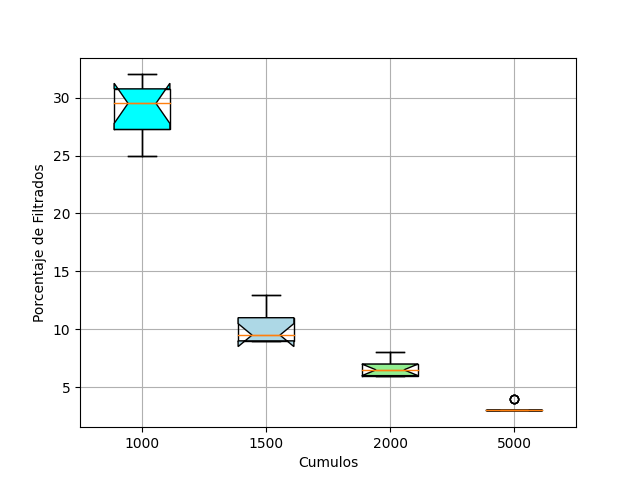
\includegraphics[width=\linewidth]{cumulos10.png}
           \caption{T=10}
           \label{f1.a}
        \end{subfigure}
 \begin{subfigure}[b]{0.90\linewidth}
           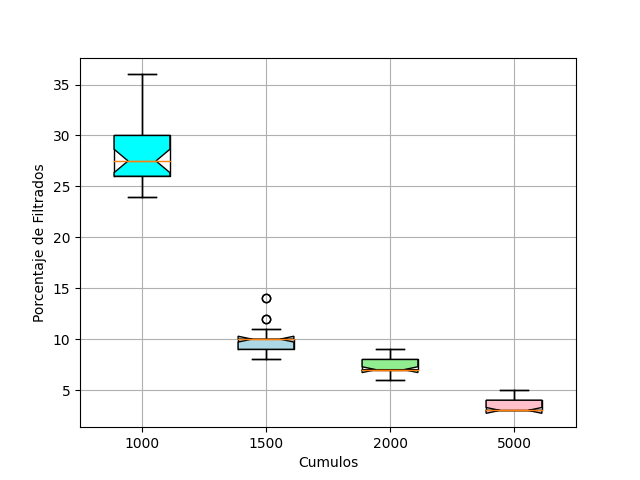
\includegraphics[width=\linewidth]{cumulos30.png}
           \caption{T=30}
           \label{f1.b}
        \end{subfigure}
\caption{Porcentaje de filtraci\'on en iteraciones de 10 y 30}
        \label{f1}
\end{figure}

\begin{figure}[H]
       \centering
        \begin{subfigure}[b]{0.90\linewidth}
            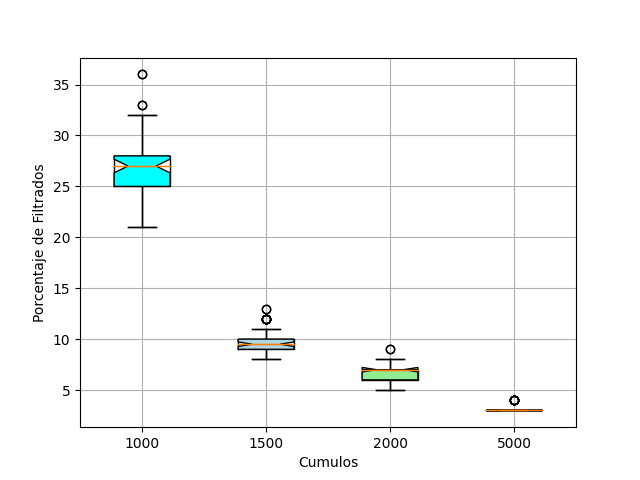
\includegraphics[width=\linewidth]{cumulos50.png}
            \caption{T=50}	
            \label{f2.a}
        \end{subfigure}
\begin{subfigure}[b]{0.90\linewidth}
            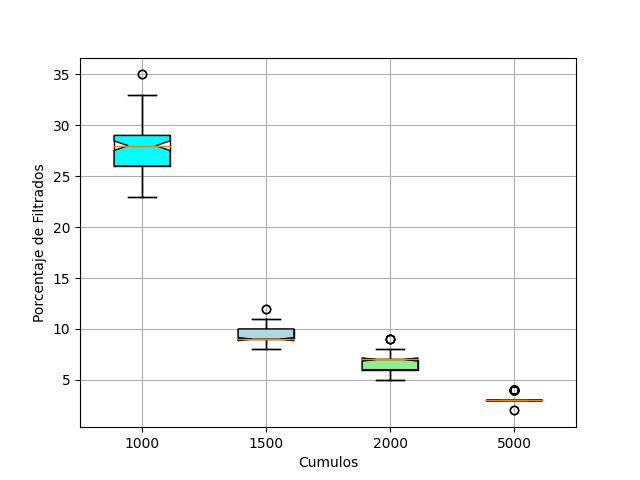
\includegraphics[width=\linewidth]{cumulos1000.png}
            \caption{T=100}
            \label{f2.b}
        \end{subfigure}
\caption{Porcentaje de filtraci\'on en iteraciones de 50 y 100}
        \label{f2}
\end{figure}

 Se observa que a mayor cantidad de c\'umulos menor ser\'a el porcentaje de filtrados, aunque comparando con las variaciones de los pasos se observa que cuando se tuvieron ``30'' iteraciones, aumento un poco m\'as el porcentaje de filtrados en comparaci\'on de las dem\'as variaciones.

\section{Conclusi\'{o}n}\label{con}

A medida que aumentamos el n\'umero de part\'iculas, se aumenta el n\'umero de c\'umulos, por lo cual es menor la cantidad de filtrados, a pesar de que estos se pueden romper, mientras mayor cantidad tengamos, mayor ser\'a la cantidad de aquellos que no pasan por el filtro, es decir compar\'andolos con el valor critico ``c'', aquellos que son iguales o mayores, no se filtrara, por lo tanto es menor el porcentaje de filtrado en estos casos.

  \bibliography{P8}
  \bibliographystyle{plainnat}
\end{document}